\documentclass[11pt]{cernrep}
\usepackage{graphicx,epsfig}
\bibliographystyle{lesHouches}
\begin{document}


\title{Recasting activities at LH2017}

\author{L. Perrozzi$^1$, fabio.maltoni@uclouvain.be, sabine.kraml@gmail.com, gabriel.facini@cern.ch, D.Grellscheid@gmail.com, ssekmen@cern.ch, J.Butterworth@ucl.ac.uk, nishita.desai@umontpellier.fr, andy.buckley@cern.ch, fuks@lpthe.jussieu.fr, eric.conte@iphc.cnrs.fr, peter.richardson@durham.ac.uk, luca.perrozzi@cern.ch, olivier.mattelaer@uclouvain.be, Pasquale.Musella@cern.ch, andre.lessa@cern.ch, alexandra.oliveira@cern.ch, ursula.laa@lpsc.in2p3.fr, kristin.lohwasser@cern.ch, thrynova@mail.cern.ch, efe.yazgan@cern.ch, philippe.gras@cern.ch, sylvain@ift.unesp.br}
\institute{
$^1$IPA at ETH Zurich, Switzerland
\\
$^2$Tate Gallery of Fundamental Research,  Trunka
}

\maketitle

\begin{abstract}
We examine Recasting activities at LH2017.
\end{abstract}

\section{INTRODUCTION}
\subsection{General Activities}
\begin{itemize}
\item Feasibility study of the implementation/portability of complicated MVA techniques (BDT, NN,…) into the analyses
\item Improvement of results and recastability: how to provide correlations signal systematics, possibility of providing a few key observables unfolded.
\item Comparison of between DELPHES results and simple object smearing.
\item Trying out the use of particle-level measurements to constrain model models
\end{itemize}

\subsection{Formats}
Object efficiency tables : which format (HEPDATA?)

\subsection{Benchmarking/Comparisons}

\begin{itemize}
\item Implementation of analyses of increasing complexity in the Analysis Description Format (LHADA Proposal) and in (BSM) Rivet and their comparison.
\item Choose an analysis of ATLAS or CMS which has cutflow and detector effects provided in some form, and possibly is already been implemented in the recasting codes CheckMate/MadAnalysis/Rivet/ATOM/.
\item Implement the same analysis in LHADA and then use the dedicated parsers to provide the analysis for the recasting codes.
\item Reproduce the NP interpretation of the original paper (=validation implementation).
\item Recast the analysis for an other new physics model and compare the results.
\item Go to point one and choose a more complicated analysis…
\end{itemize}
it would be interesting to see how Delphes performance looks without analysis-specific cards, since a lot of people (outside the “big” recasting groups) are using it that way.

\subsection{How to validate the analyses}
\begin{figure}
\begin{center}
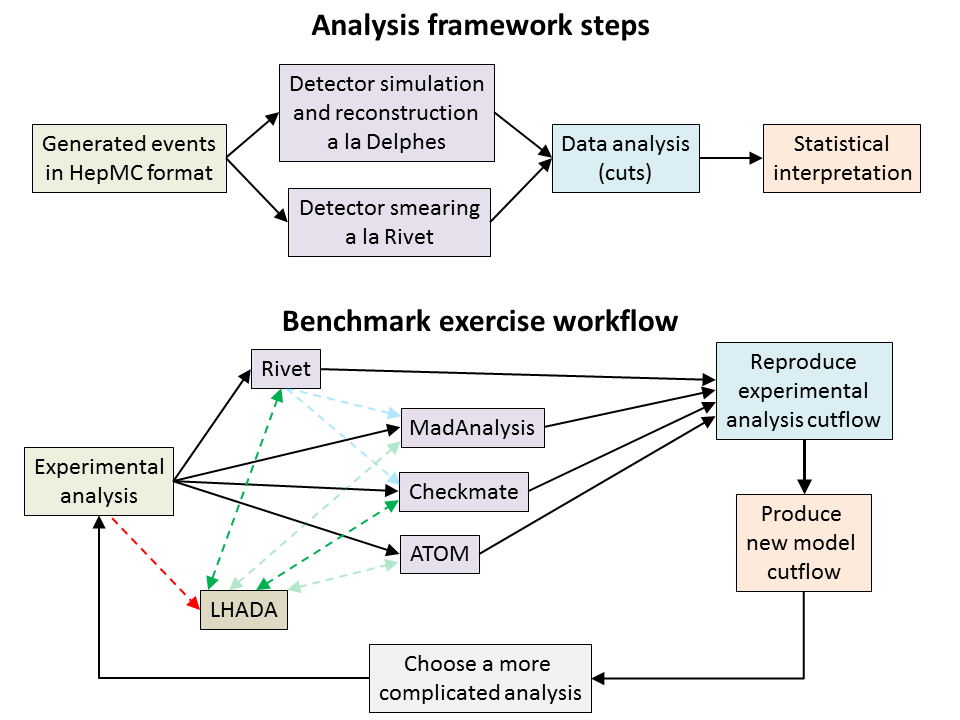
\includegraphics[width=0.5\textwidth]{figures/lhada_benchmarking_excersise.png}
 \caption{Search reach for the $\mu \gamma {\not\!\!E}_{T}$ signal
(as defined in the
   text) for
   300 fb$^{-1}$ integrated luminosity  at the LHC.
}
\label{search}
\end{center}
\end{figure}


\subsection{Analysis proposals}

\subsubsection{arxiv:1605.03814 - Jets+MET - ATLAS - 13 TeV}

Experimental cards –> Ben. The procedure for event generation is depicted multijet.pdf (Section 02), the three parameter_cards are given param_cards.tgz and the Pythia configuration files are py8_scripts.tgz
Plot conditions: HEPMC (after jet clustering), HEPMC + cuts, HEPMC + Detector effects, HEPMC + Detector effects + cuts
Plots: pT of 1j, 2j and 3j, and MET: range [0,1] TeV, 50 bins
Plots: eta of 1j, 2j and 3j: range [-5,5], 20 bins
Analysis cutflows: Tables 1-7 in http://atlas.web.cern.ch/Atlas/GROUPS/PHYSICS/PAPERS/SUSY-2015-06/
100K HepMC events with MG5_aMC LO, masses: gluino 1600, N1 0 –> Olivier+Nishita https://cernbox.cern.ch/index.php/s/3Ci4I2cgQmKwDXt
Results: here
?K HepMC events with MG5_aMC LO, masses: gluino 1100, N1 700 –> Olivier+Nishita
Results: here
LHADA implementation: https://github.com/lhada-hep/lhada/tree/master/analyses/ATLASSUSY1605.03814

\subsubsection{arxiv:1704.03848 - Monophoton - ATLAS - 13 TeV}
Cutflow: https://atlas.web.cern.ch/Atlas/GROUPS/PHYSICS/PAPERS/EXOT-2016-32/

\subsubsection{CMS-SUS-16-039 - 3 leptons + MET - CMS - 13 TeV} - (Now superseded by paper: http://cms-results.web.cern.ch/cms-results/public-results/publications/SUS-16-039/index.html)  (BDT with ~15 inputs; eff. 20-90%). Cutflows: http://cms-results.web.cern.ch/cms-results/public-results/preliminary-results/SUS-16-039/index.html Efficiencies: https://twiki.cern.ch/twiki/bin/view/CMSPublic/SUSMoriond2017ObjectsEfficiency

\subsubsection{arxiv:1706.04402 - 1 lepton + MET + Jets (>=1b) - CMS - 13 TeV} (topness variable?)

\section{Results}

\section*{CONCLUSIONS}


\section*{ACKNOWLEDGEMENTS}
K. Slane would like to thank CERN and LAPTh for hospitality offered
during which some of the work contained herein was performed.

\bibliography{sample_bib}

\end{document}
